\chapter{Finding Optimal Bandwidth}

\section{Cross-Validation Estimator}

The cross-validation estimator is defined as
\begin{equation*}
    \hat{J}(h) = \int \hat{f}(x)^2 dx - \frac{2}{n}\sum_{i=1}^{n}\hat{f}_{(-i)}
    (X_i), 
\end{equation*}
where $\hat{f}_{(-i)}$ is the histogram estimator after removing the $i$th
observation.

\subsection*{(a)}

We can write the histogram estimator $\hat{f}(x)$ as 
\begin{equation*}
  \begin{aligned}
    \hat{f}(x) &= \sum_{k=1}^{m}\frac{\hat{p_k}}{h}\mathbb{I}    [x\in B_k] \\
    &= \sum_{k=1}^{m}\frac{v_k}{nh}\mathbb{I}[x\in B_k].
  \end{aligned}
\end{equation*} 
Hence,
\begin{equation}
  \begin{aligned}
    \int\hat{f}(x)^2 dx &= \int \left(\sum_{k=1}^{m}\frac{v_k}{nh}\mathbb{I}[x\in
    B_k]\right)^2 dx \\
    &= \sum_{j=1}^{m} \int_{B_j}\left(\sum_{k=1}^{m}\frac{v_k}{nh}\mathbb{I}[x\in
    B_k]\right)^2 dx + 0 \\
    &= \sum_{j=1}^{m}\int_{B_j}\left(\frac{v_j}{nh}\right)^2 dx \\
    &= \sum_{j=1}^{m} \frac{(v_j)^2}{n^2 h^2}h \\
    &= \frac{1}{n^2 h}\sum_{j=1}^{m}(v_j)^2.
  \end{aligned}
  \label{eq1.1}
\end{equation}
This is the required result.

\subsection*{(b)}

Suppose $X_i\in B_j$. Then on removing $X_i$, the number of points in $B_j$ is
$v_j-1$ and the total number of points is $n-1$. Hence, $\hat{f}_{(-i)}(X_i) =
\frac{(v_j-1)}{(n-1)h}$. Using this result, 
\begin{equation}
  \begin{aligned}
    \sum_{i=1}^{n} \hat{f}_{(-i)}(X_i) &= \sum_{i=1}^{n}\sum_{j=1}^{m} \frac{v_j-
    1}{(n-1)h}\mathbb{I}[X_i\in B_j] \\
    &= \sum_{j=1}^{m}\sum_{i=1}^{n} \frac{v_j-1}{(n-1)h}\mathbb{I}[X_i\in B_j] \\
    &= \sum_{j=1}^{m} \frac{v_j-1}{(n-1)h}\cdot v_j \\
    &= \frac{1}{(n-1)h}\sum_{j=1}^{m} (v_j^2 - v_j).
  \end{aligned}
  \label{eq1.2}
\end{equation}
This is the second part. We can combine the \ref{eq1.1} and \ref{eq1.2} parts to
write the cross-validation estimator as 
\begin{equation*}
  \hat{J}(h) = \frac{2}{(n-1)h} - \frac{n+1}{(n-1)h}\sum_{j=1}^{m} \hat{p}_j^2
\end{equation*}

\section{ Using the Cross-Validation Estimator}

\subsection*{(a)}
The probabilities were calculated using \texttt{numpy.histogram} function. The
estimated probabilities $\hat{p}_j$ for all the bins are:
\begin{center}
  \begin{tabular}{ | c | c |}
    \hline
    \textbf{Bin} & \textbf{$\hat{p}_j$} \\
    \hline
    1 & 0.20588235 \\
    2 & 0.48823529 \\
    3 & 0.04705882 \\
    4 & 0.04117647 \\
    5 & 0.13529412 \\
    6 & 0.05882353 \\
    7 & 0.00588235 \\
    8 & 0.0 \\
    9 & 0.01176471 \\
    10 & 0.00588235 \\
    \hline
  \end{tabular}
\end{center}
Using the obtained values, the histogram was plotted using the
\texttt{matplotlib.pyplot.hist} function. The histogram plot can be found in
\texttt{images/10binhistogram.png}.

\begin{figure}[H]
  \centering
  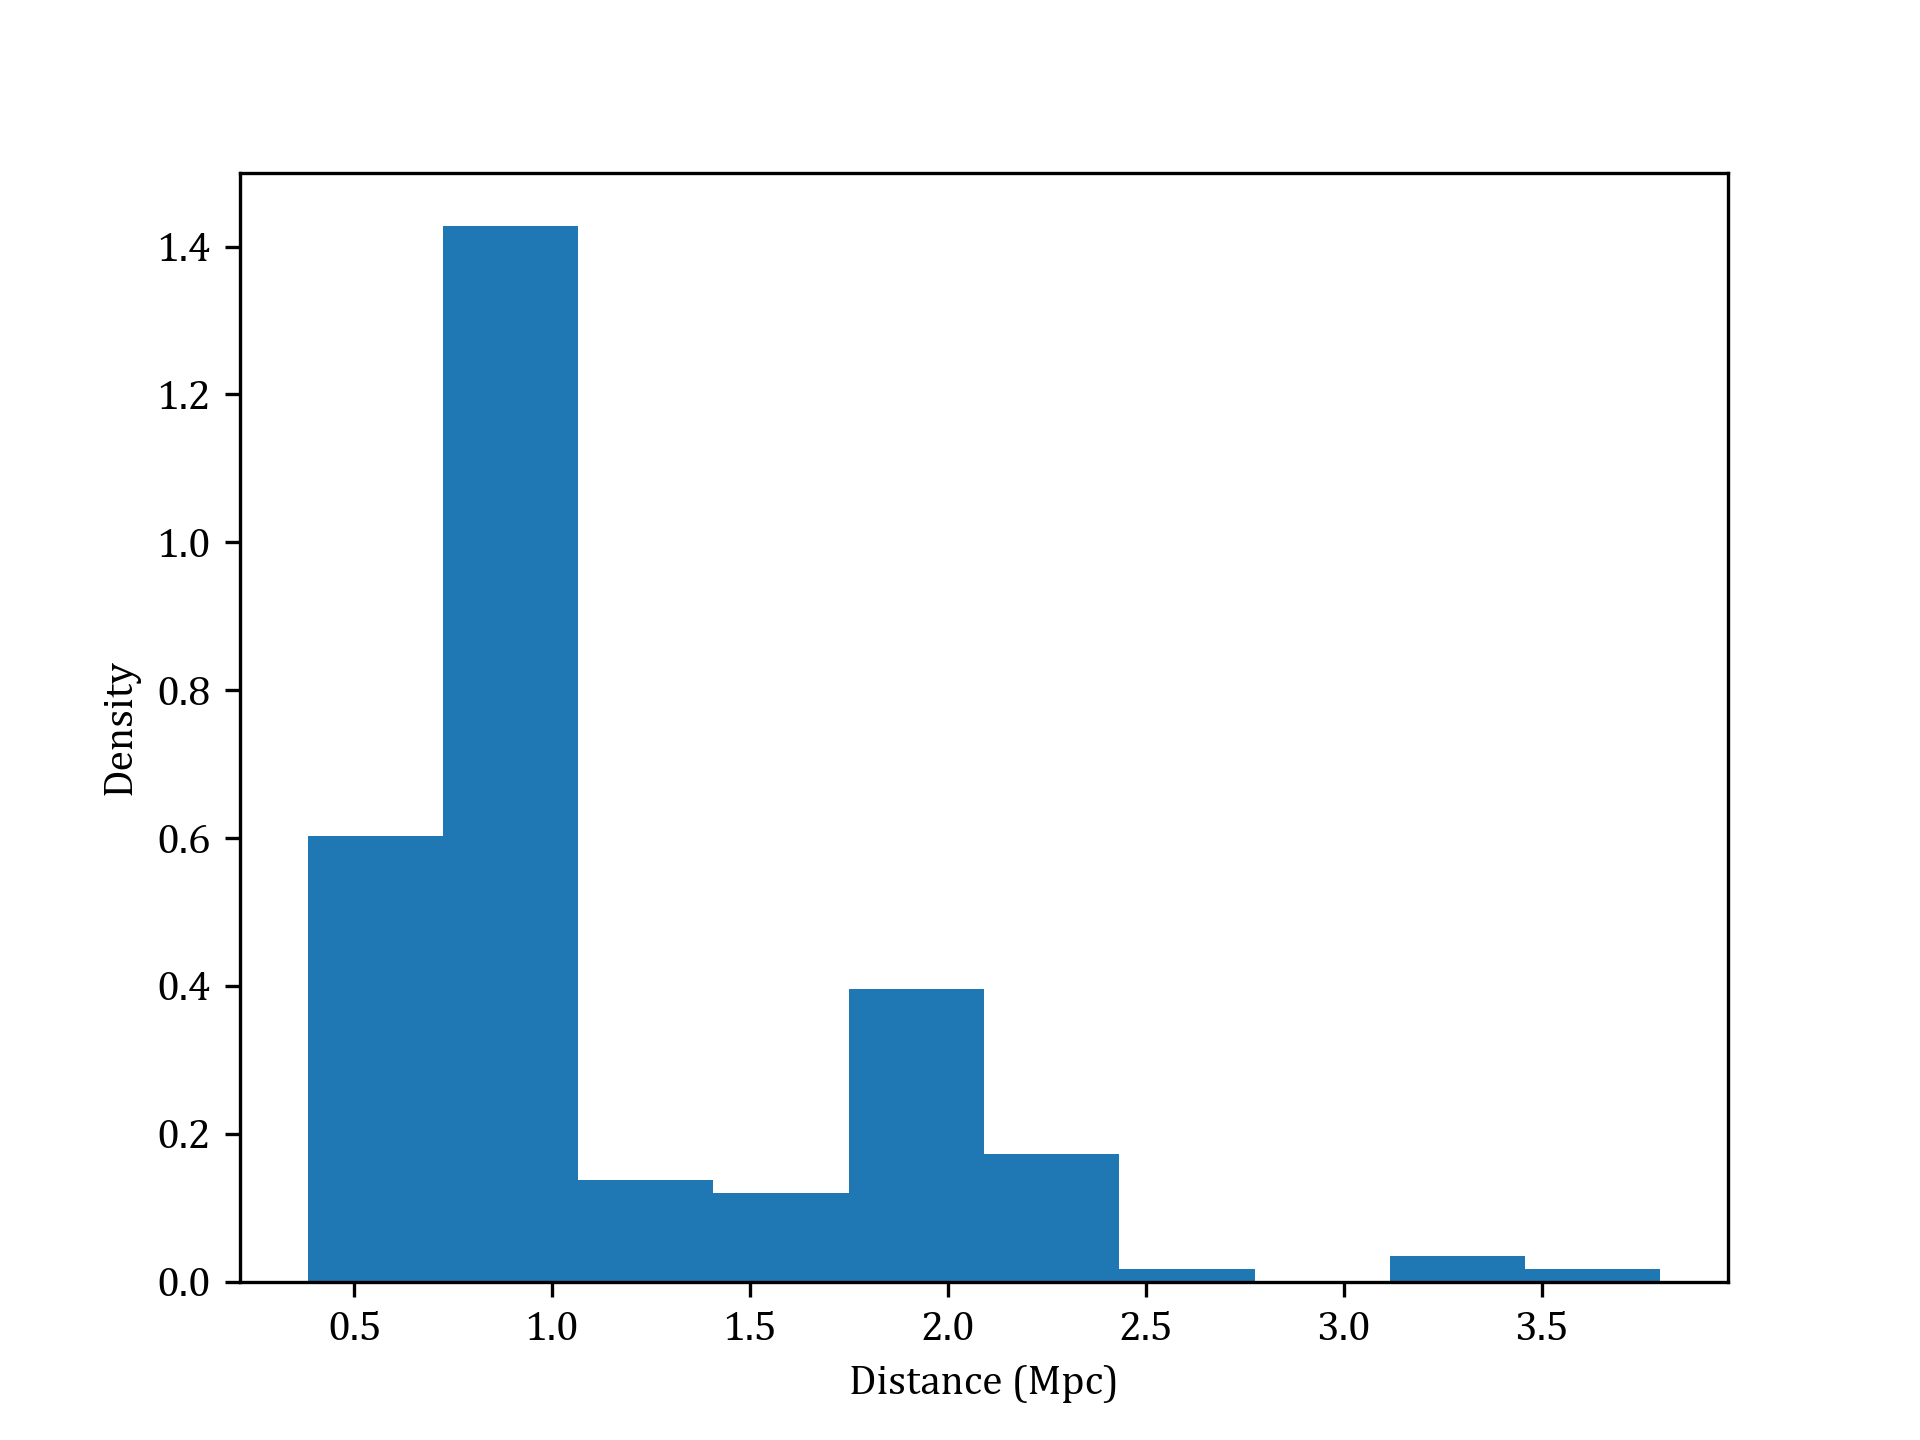
\includegraphics[width=0.5\textwidth]{assets/images/10binhistogram.png}
  \caption{10 Bin Histogram}
\end{figure}


\subsection*{(b)}

The probability distribution is \textbf{oversmoothed}. Lower values of $h$ yield
a lower cross-validation score.

\subsection*{(c)}

The cross-validation score for the number of bins from 1 to 1000 was calculated
using: \texttt{numpy.histogram}, \texttt{numpy.square} and \texttt{numpy.sum}
functions. The plot of cross-validation score versus $h$ can be found in
\texttt{images/crossvalidation.png}

\begin{figure}[H]
  \centering
  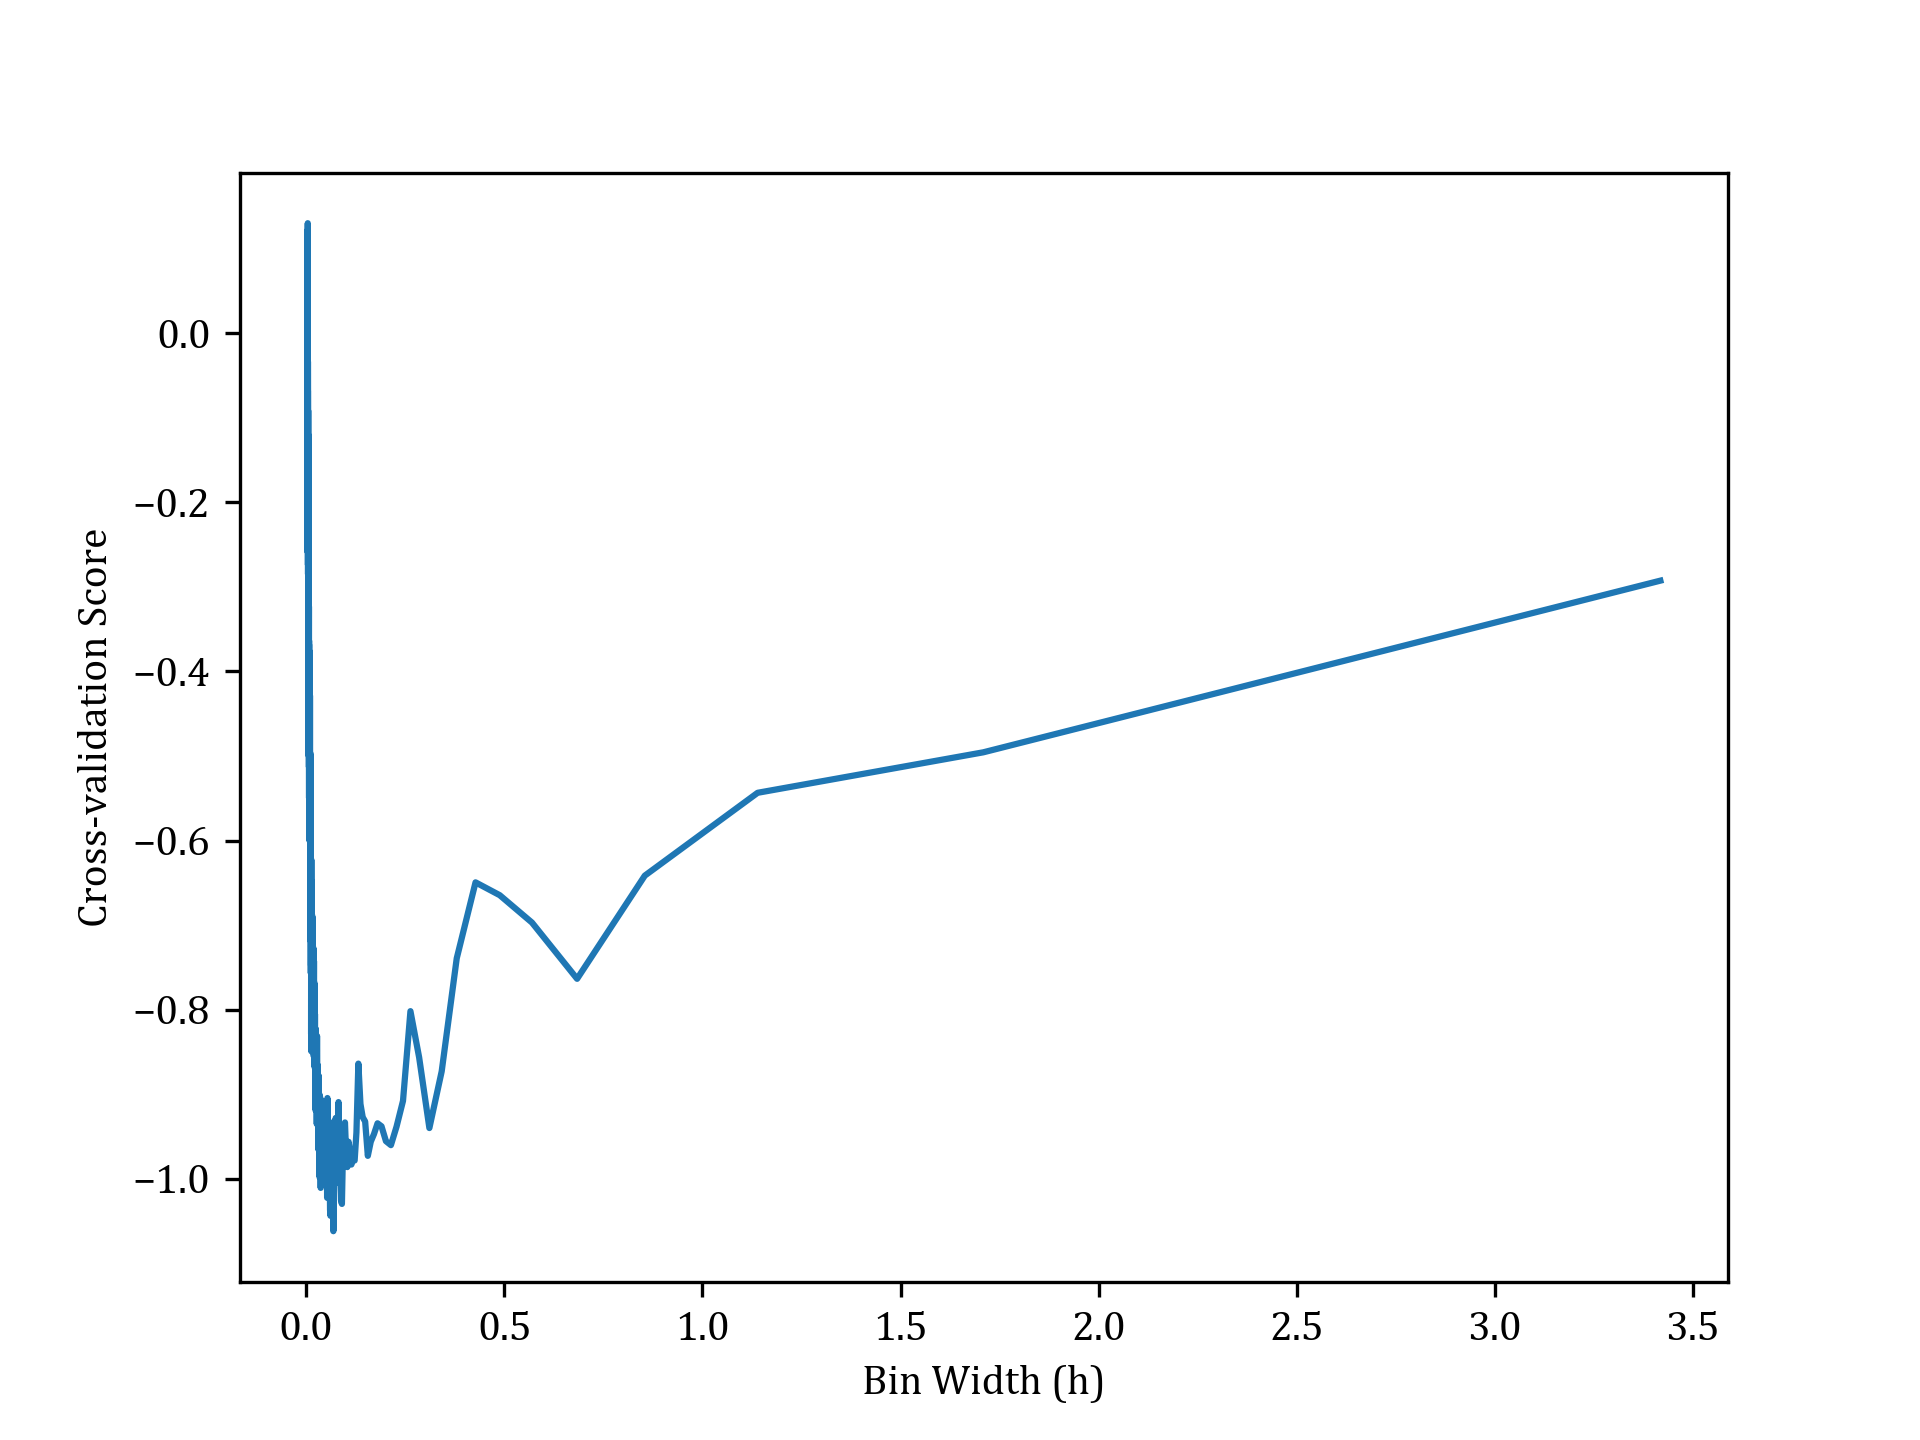
\includegraphics[width=0.5\textwidth]{assets/images/crossvalidation.png}
  \caption{Cross Validation}
\end{figure}

\subsection*{(d)}

The optimal bin width is the value of $h$ for which the cross-validation score is
minimum. From the plot, this corresponded to 50 bins, for which the value of $h$
is \textbf{0.06835999} Mpc.

\subsection*{(e)}

The histogram with optimal value $h^* = 0.06835999$ is present in
\texttt{images/optimalhistogram.png}.

\begin{figure}[H]
  \centering
  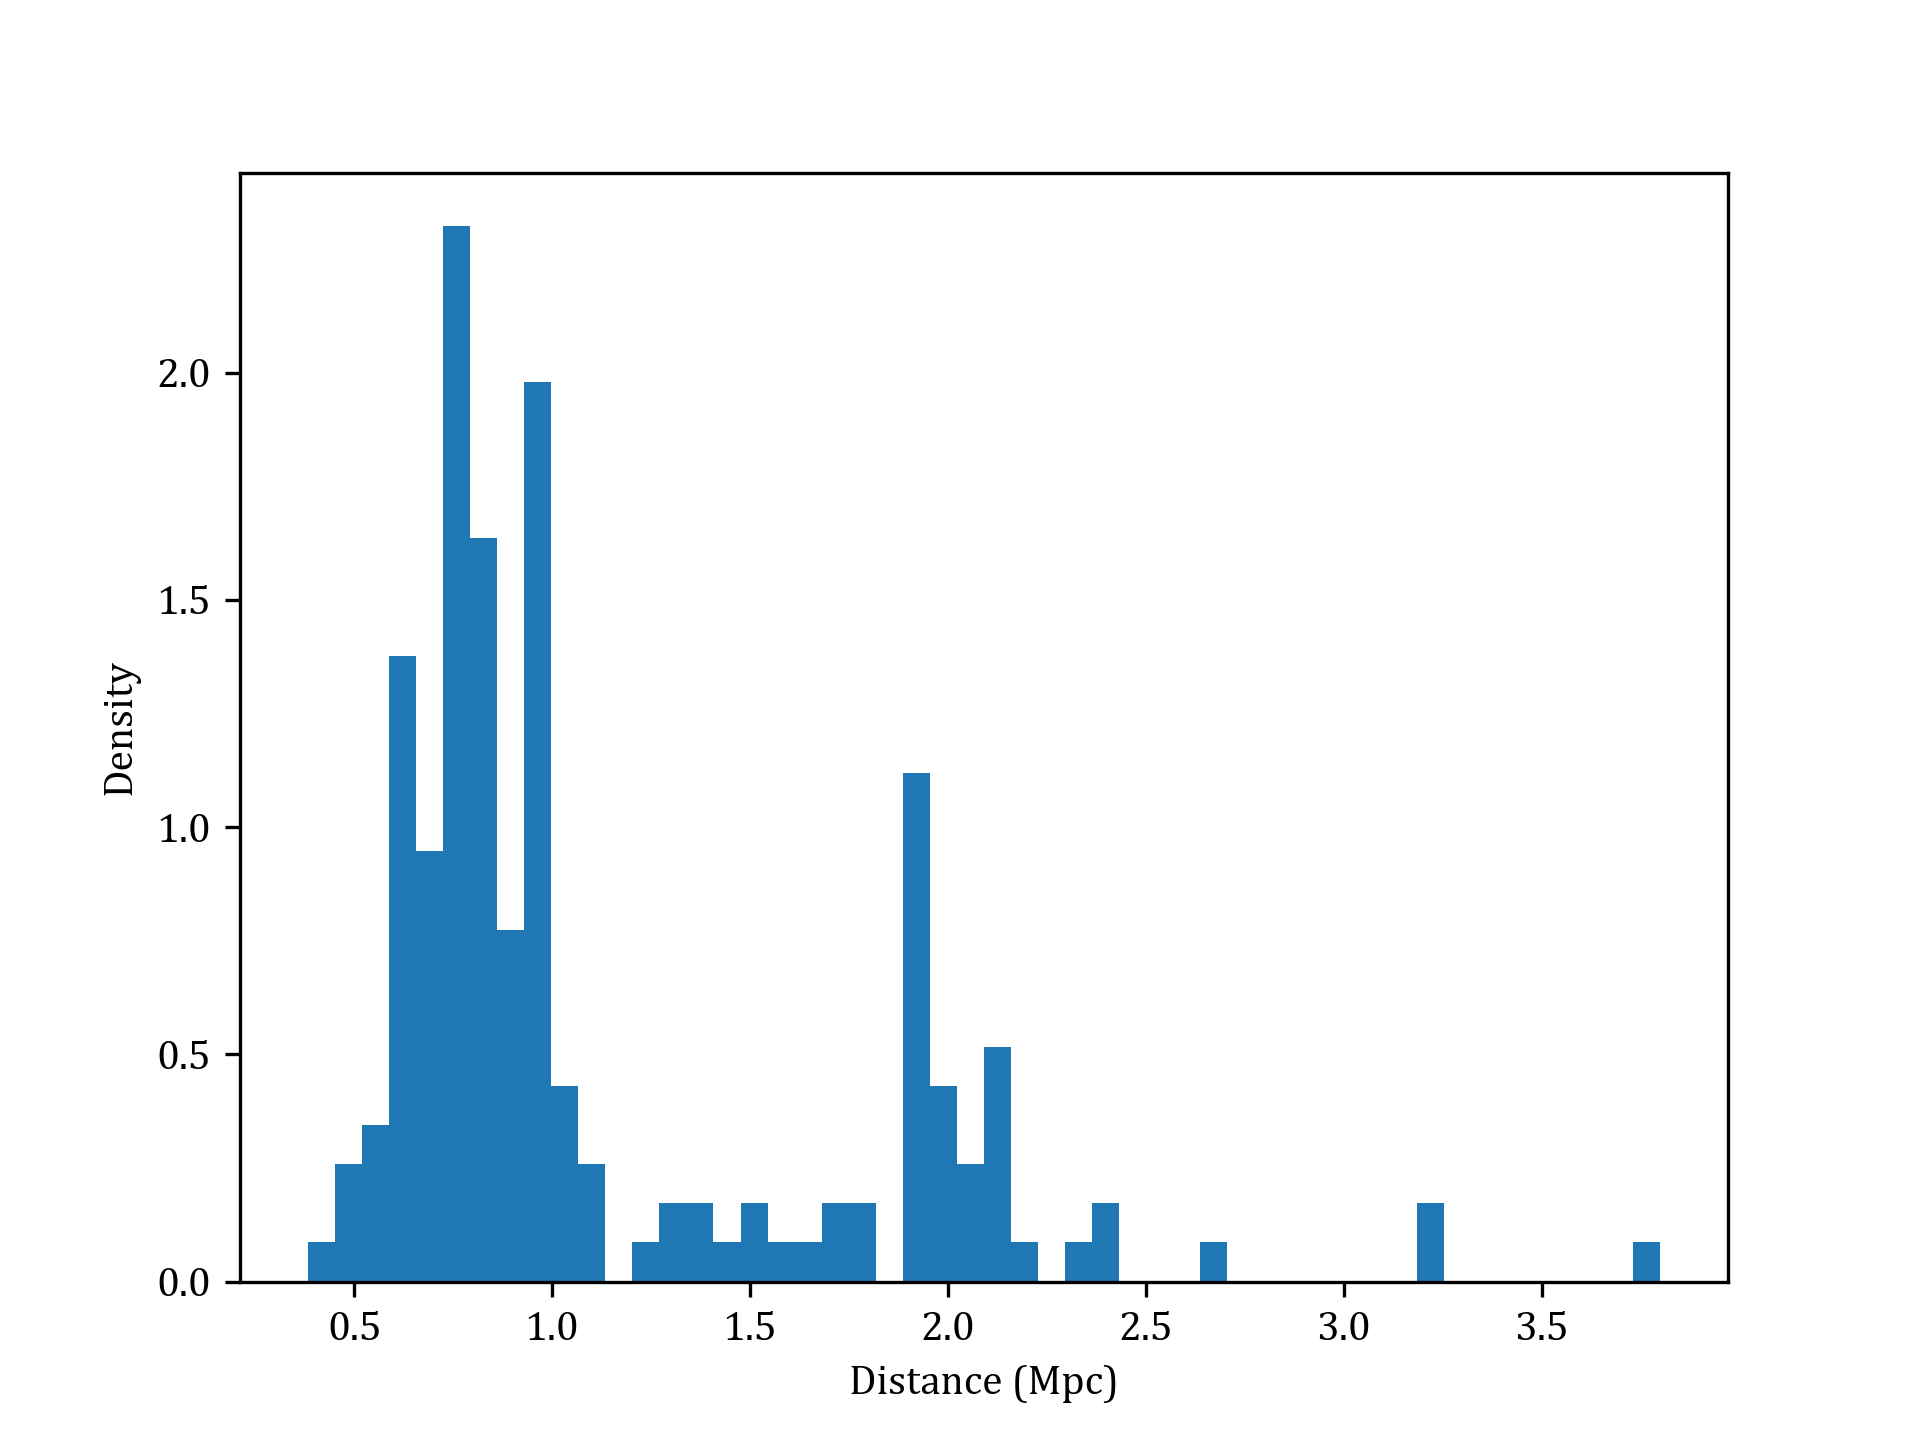
\includegraphics[width=0.5\textwidth]{assets/images/optimalhistogram.png}
  \caption{Cross Validation}
\end{figure}

\subsection*{(f)}

The code for all the parts is present in \texttt{code/1.py}. 
